\section{异常检测}
\label{sec:chapter13}

\subsection{多元正态分布}

多元正态分布的概率密度函数为：
\[
p(x;\mu,\Sigma)=\frac{1}{(2\pi)^{n/2}|\Sigma|^{1/2}}\exp\left(-\frac{1}{2}(x-\mu)^T\Sigma^{-1}(x-\mu)\right)
\]
其中，$x\in\mathbb R^n$ 是 $n$ 维随机变量，$\mu\in\mathbb R^n$ 是 $x$ 的均值，$\Sigma\in\mathbb R^{n\times n}$ 是协方差矩阵。均值决定分布的中心位置，协方差矩阵则描述各维度的变化范围以及不同维度之间的相关关系。

特别地，当 $x$ 的各个维度不相关、协方差矩阵为对角矩阵时，联合概率密度可以分解为各分量概率密度的乘积，即：
\[
p(x;\mu,\Sigma)=\prod_{i=1}^np(x_i;\mu_i,\sigma_i^2)
\]


\subsection{异常检测}

异常检测的基本思想是先利用正常样本估计数据通常出现的区域，再将概率很低的新样本视为异常。设正常数据集为 $\{x^{(1)},x^{(2)},\ldots,x^{(m)}\}$，可以使用样本均值和协方差矩阵构建多元正态分布：
\begin{gather*}
\mu=\frac{1}{m}\sum\limits_{i=1}^mx^{(i)}\\
\Sigma=\frac{1}{m}\sum\limits_{i=1}^m(x^{(i)}-\mu)(x^{(i)}-\mu)^T\\
p(x;\mu,\Sigma)=\frac{1}{(2\pi)^{n/2}|\Sigma|^{1/2}}\exp\left(-\frac{1}{2}(x-\mu)^T\Sigma^{-1}(x-\mu)\right)
\end{gather*}
如果不希望估计完整协方差矩阵，也可以进一步假设 $x$ 的各维度相互独立，分别拟合每一维的正态分布，再取各概率密度之积：
\[
p(x;\mu,\Sigma)=\prod_{i=1}^np(x_i;\mu_i,\sigma_i^2)
\]

\begin{note}
后者计算更快，且允许 $m<n$ 的情况；而前者在 $m<n$ 时 $\Sigma$ 不可逆。
\end{note}

模型建立后，对于待检测样本 $x$，计算其在所拟合分布下的概率密度。若 $p(x;\mu,\Sigma)$ 小于阈值 $\varepsilon$，说明该样本在正常数据中出现的可能性很低，因此将其判定为异常；否则判定为正常。

若部分数据带有是否异常的标注，可以将数据划分为训练集、验证集和测试集。训练集主要包含正常样本，用于估计 $\mu$ 和 $\Sigma$ 并建立概率模型；验证集同时包含正常与异常样本，用于比较不同阈值并选择 $\varepsilon$；测试集同样包含两类样本，但只用于最终评估。

\begin{note}
异常检测通常属于类别极不平衡的问题，正常样本远多于异常样本。此时即使把所有样本都预测为正常，也可能得到很高的准确率，因此准确率并不是合适的主要指标。应使用 $\text{precision},\text{recall},\text{F1}$ 等指标综合评估异常样本的识别效果。
\end{note}


\subsection{代码实现}

根据训练集构建的二元正态分布如下：

\begin{figure}[H]
    \centering
    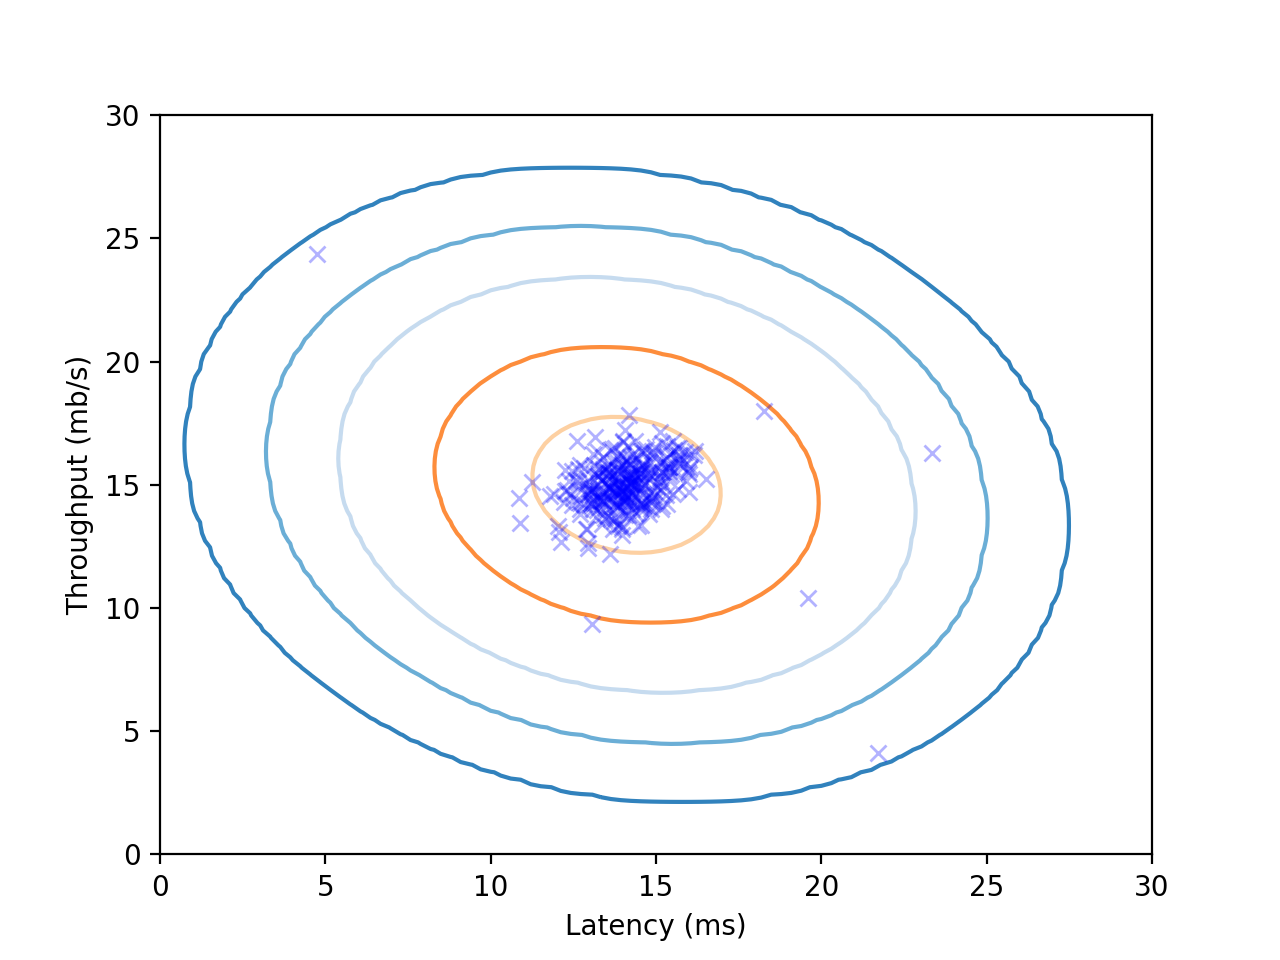
\includegraphics[width=0.5\linewidth]{figs/Chap_13_Figure_0.png}
\end{figure}

\begin{lstlisting}[language=Python]
Xmeans = X.mean(axis=0)
Xcov = ((X - Xmeans).T @ (X - Xmeans)) / X.shape[0]
normDist = multivariate_normal(mean=Xmeans, cov=Xcov)
\end{lstlisting}

依次尝试不同阈值，并根据验证集上的 $\text{F1}$ 选择最佳值。最终得到的最佳 $\varepsilon$ 约为 $2.72\times 10^{-5}$，此时测试集上的 $\text{F1}$ 约为 $0.75$. 

\begin{figure}[H]
    \centering
    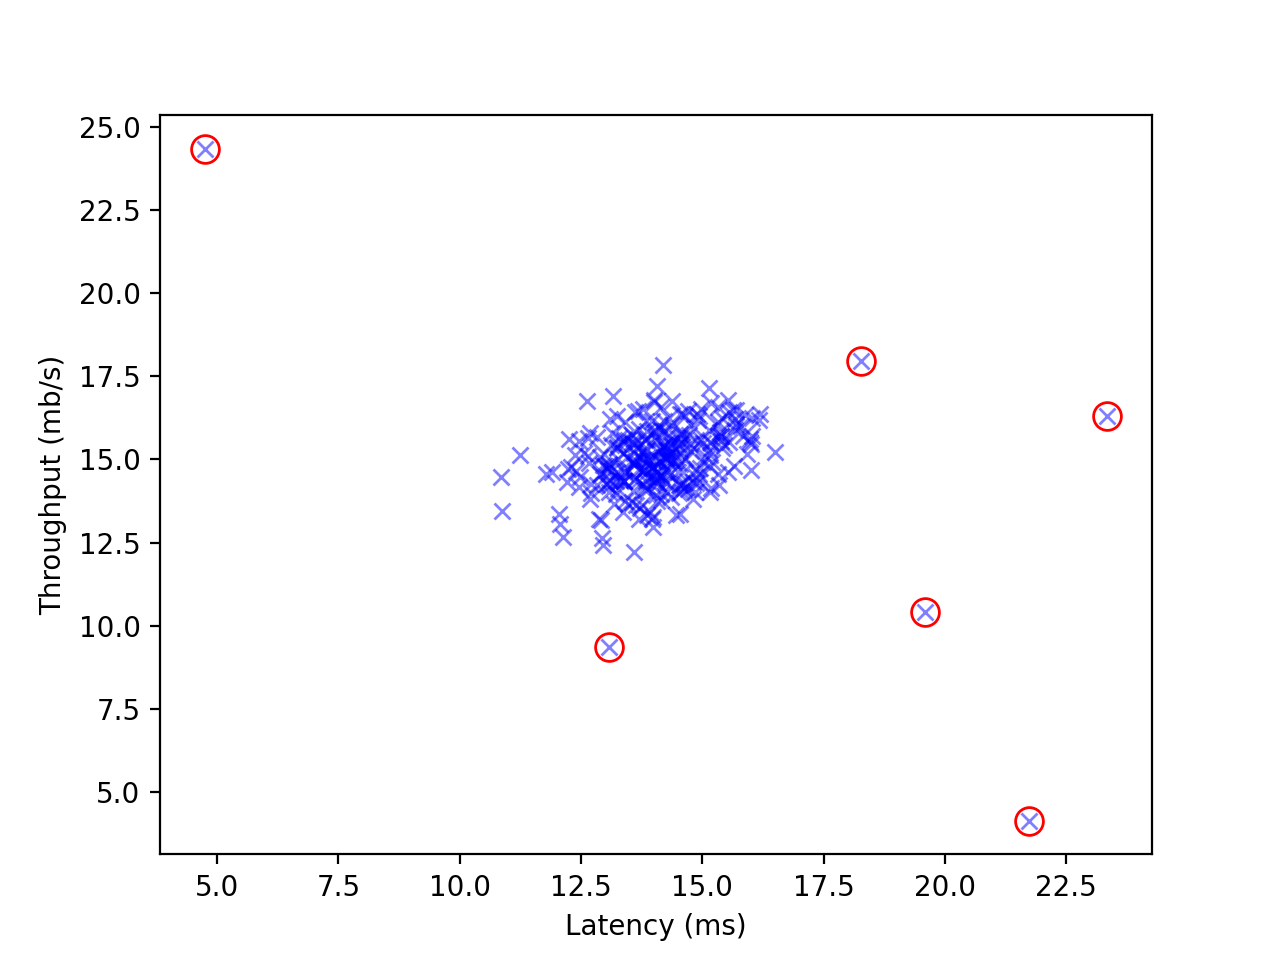
\includegraphics[width=0.5\linewidth]{figs/Chap_13_Figure_1.png}
\end{figure}
